
\section{Dataset}

\subsection{Dataset Description}
The dataset used in this study comprises structural connectivity (SC) and functional connectivity (FC) matrices 
obtained from MRI and fMRI scans, respectively. The data is categorized into three age groups: 
young (10 years old), adult (30 years old), and old (70 years old). Each age group contains data from 5 different subjects.
Both SC and FC matrices have dimensions of 200 $\times$ 200 $\times$ 5 (nodes $\times$ nodes $\times$ subjects).

\subsection{Data Loading and Preprocessing}
Data was loaded from .mat files, and matrices for different age groups (young, adult, old) were extracted and stored in separate variables of size 200 $\times$ 200 $\times$ 5 (nodes $\times$ nodes $\times$ subjects).

Preprocessed FC matrices by setting negative weights to zero and applying thresholding to remove weak connections. Applied min-max scaling to both SC and FC matrices to adjust the data within the range of [0, 1].
Visualized heatmaps and histograms of the original and preprocessed SC and FC matrices to have a better understanding of the distribution of connectivity strengths.

\begin{figure}[h!]
    \centering
    \begin{subfigure}[b]{0.45\textwidth}
        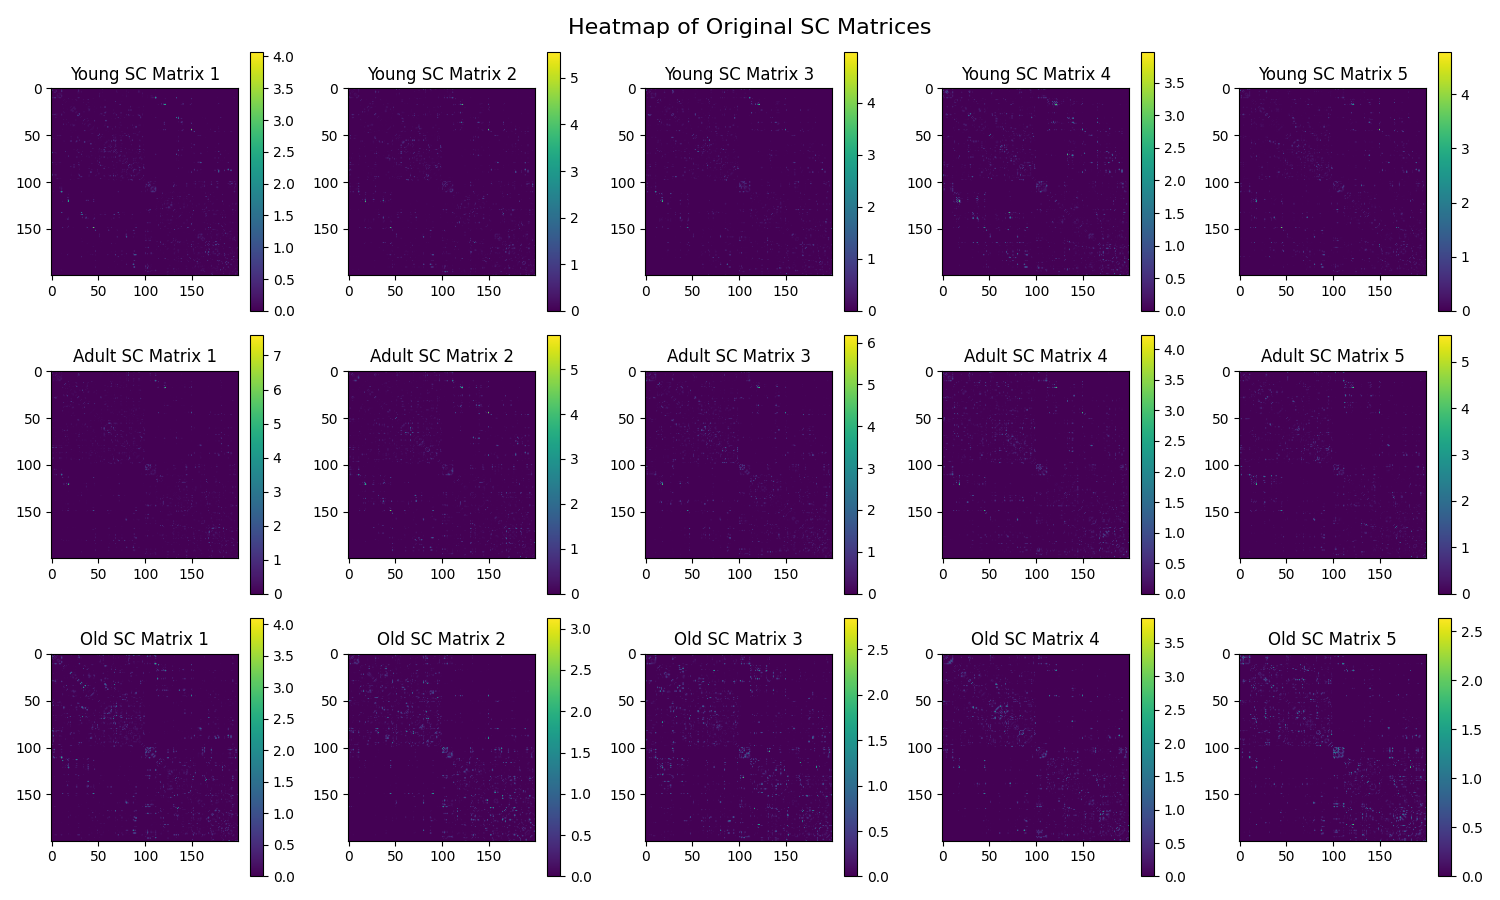
\includegraphics[width=\textwidth]{C:/Users/barbo/Desktop/thesis repo clone/thesis/Thesis Draft/figures/SC_matrices_heatmap.png}
        \caption{Heatmap of Original SC Matrices}
    \end{subfigure}
    \begin{subfigure}[b]{0.45\textwidth}
        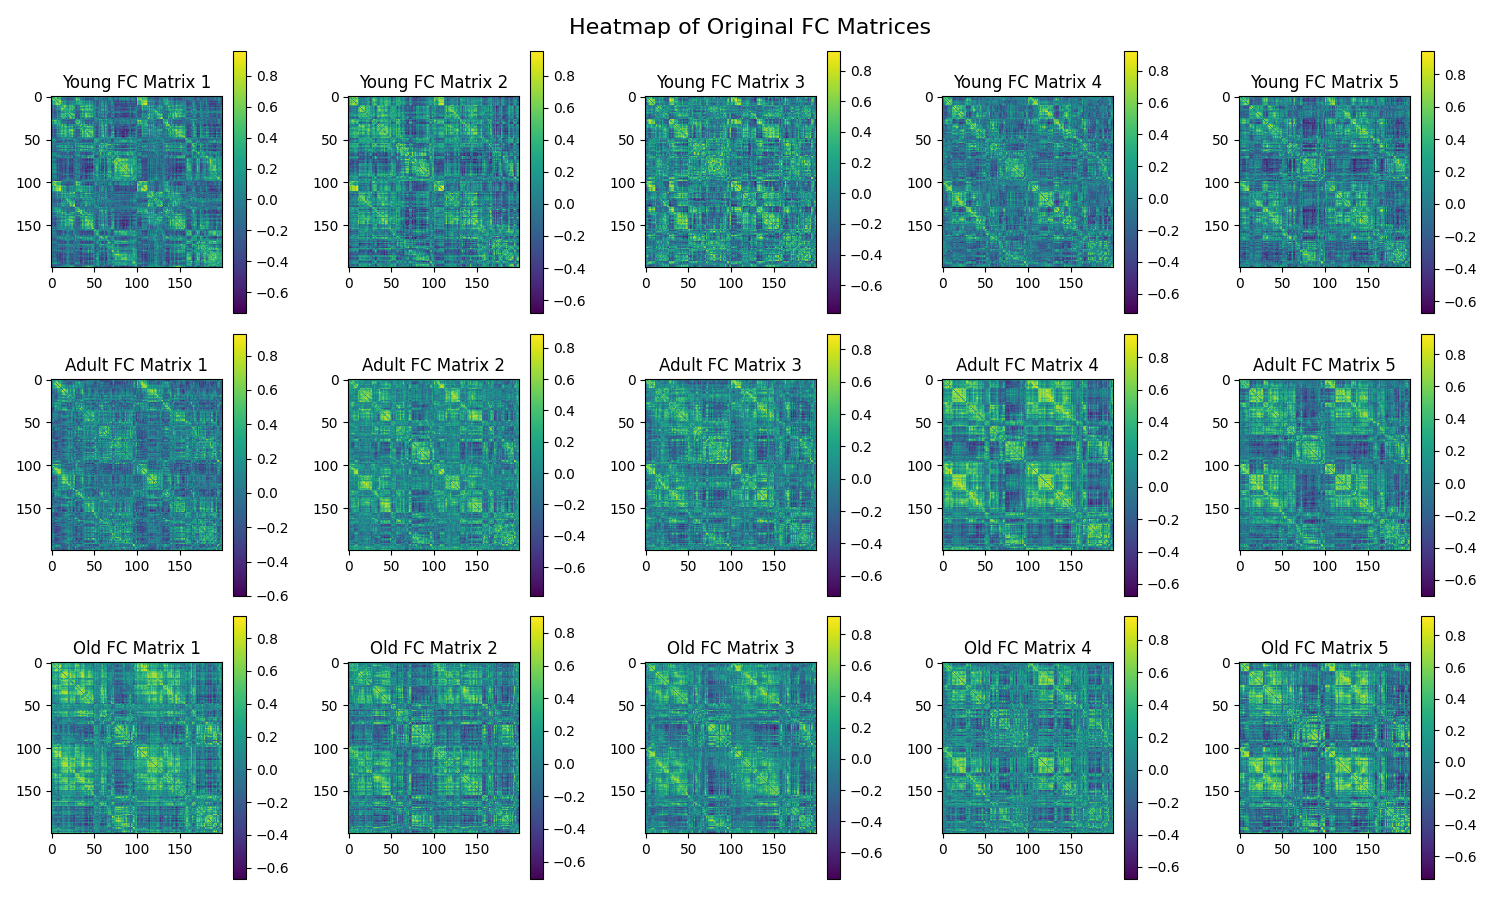
\includegraphics[width=\textwidth]{C:/Users/barbo/Desktop/thesis repo clone/thesis/Thesis Draft/figures/FC_matrices_heatmap.png}
        \caption{Heatmap of Original FC Matrices}
    \end{subfigure}
    \begin{subfigure}[b]{0.45\textwidth}
        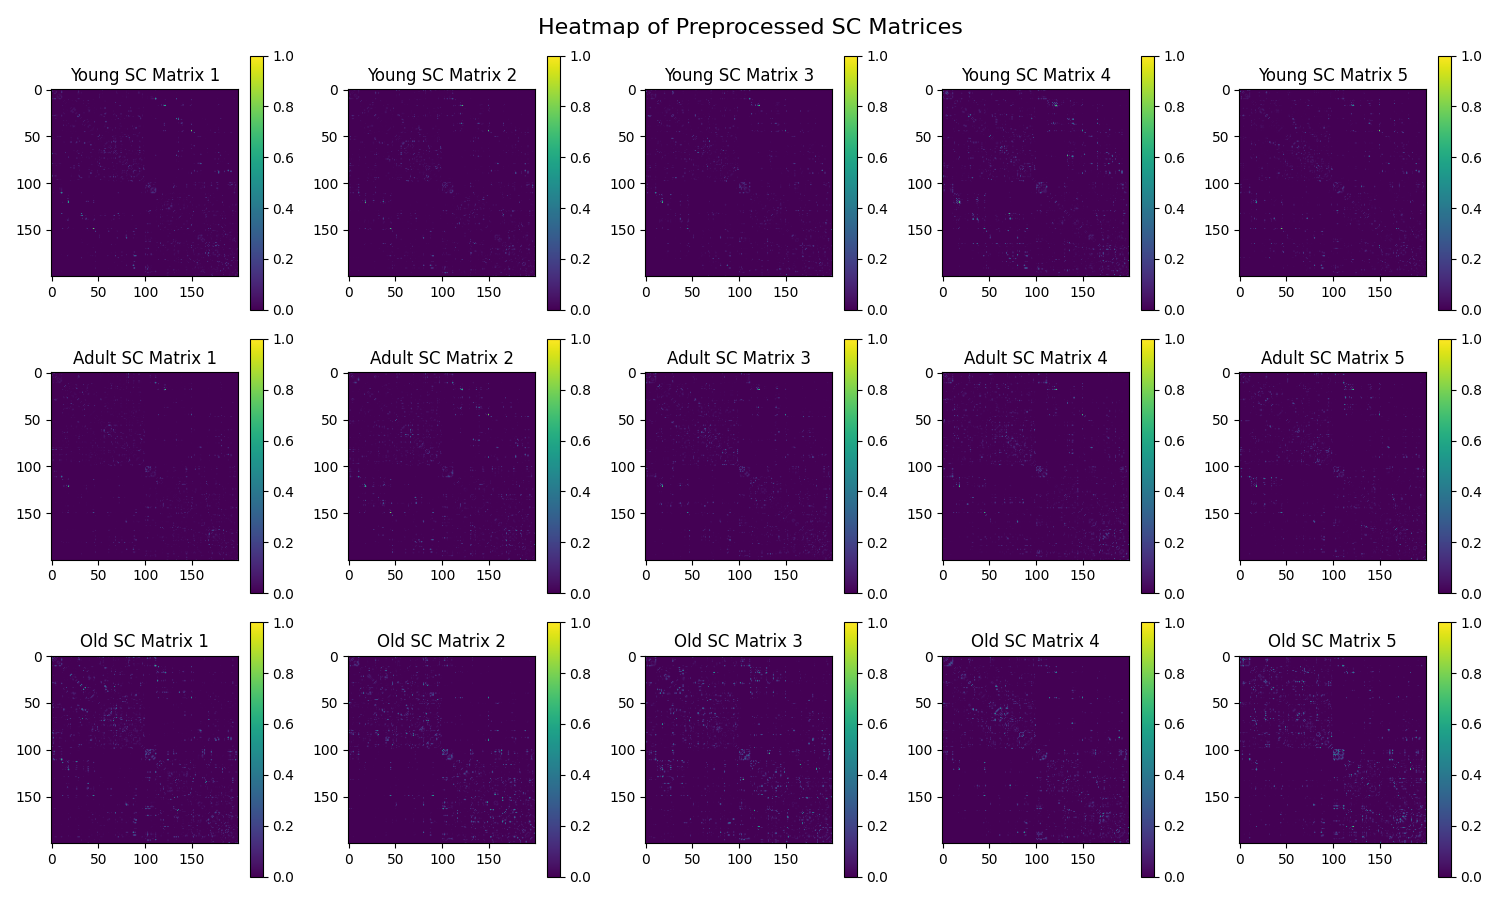
\includegraphics[width=\textwidth]{C:/Users/barbo/Desktop/thesis repo clone/thesis/Thesis Draft/figures/SC_matrices_heatmap_preprocessed.png}
        \caption{Heatmap of Preprocessed SC Matrices}
    \end{subfigure}
    \begin{subfigure}[b]{0.45\textwidth}
        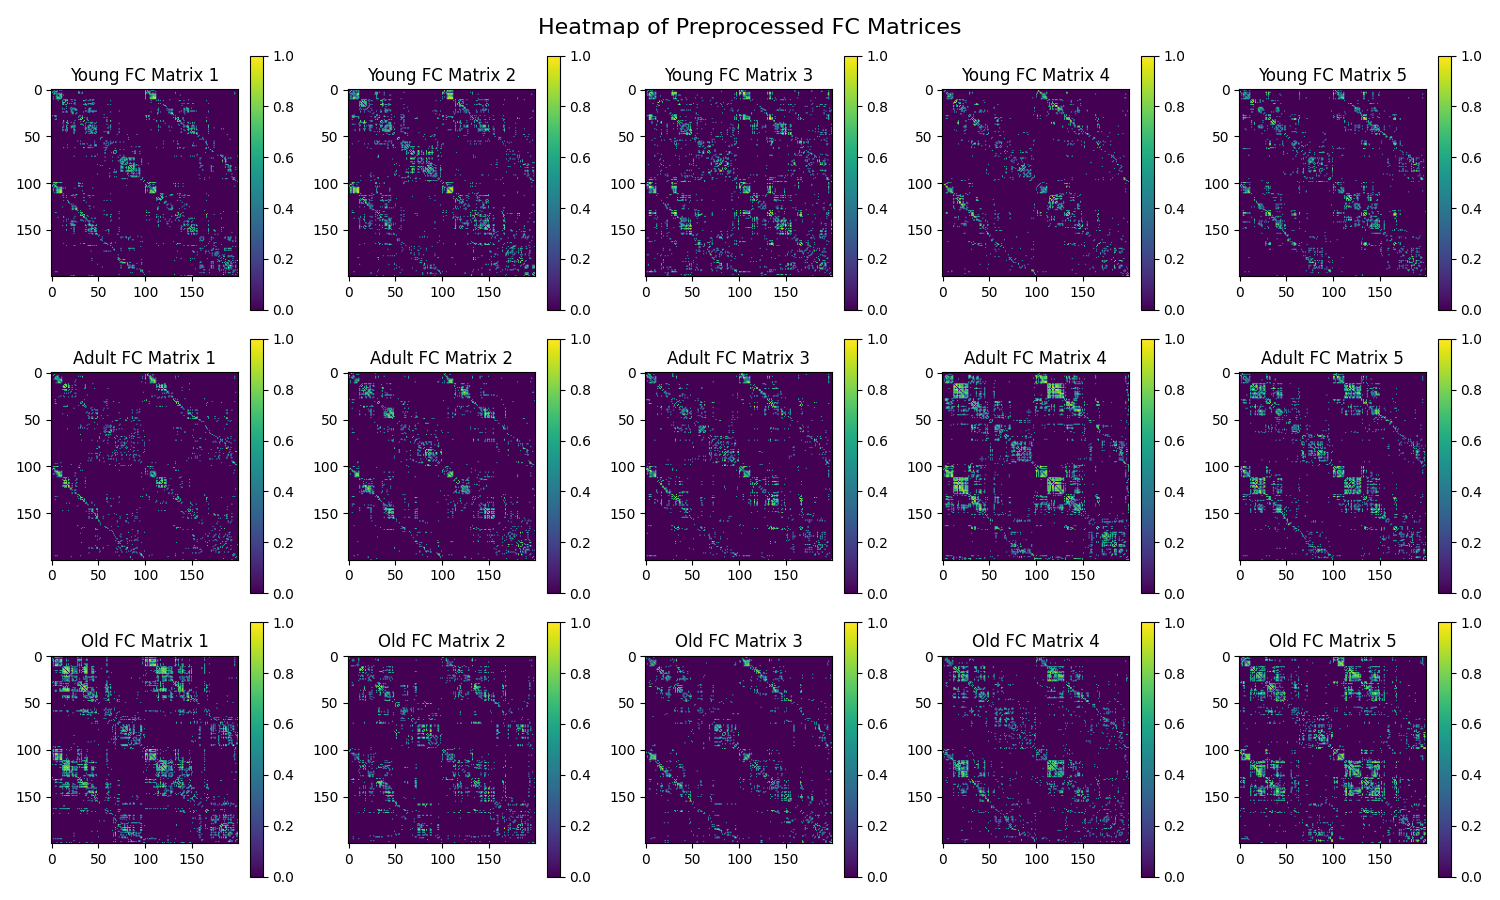
\includegraphics[width=\textwidth]{C:/Users/barbo/Desktop/thesis repo clone/thesis/Thesis Draft/figures/FC_matrices_heatmap_preprocessed.png}
        \caption{Heatmap of Preprocessed FC Matrices}
    \end{subfigure}
    \caption{Various Heatmaps of SC and FC Matrices}
\end{figure}


\begin{figure}[h!]
    \centering
    \begin{subfigure}[b]{0.45\textwidth}
        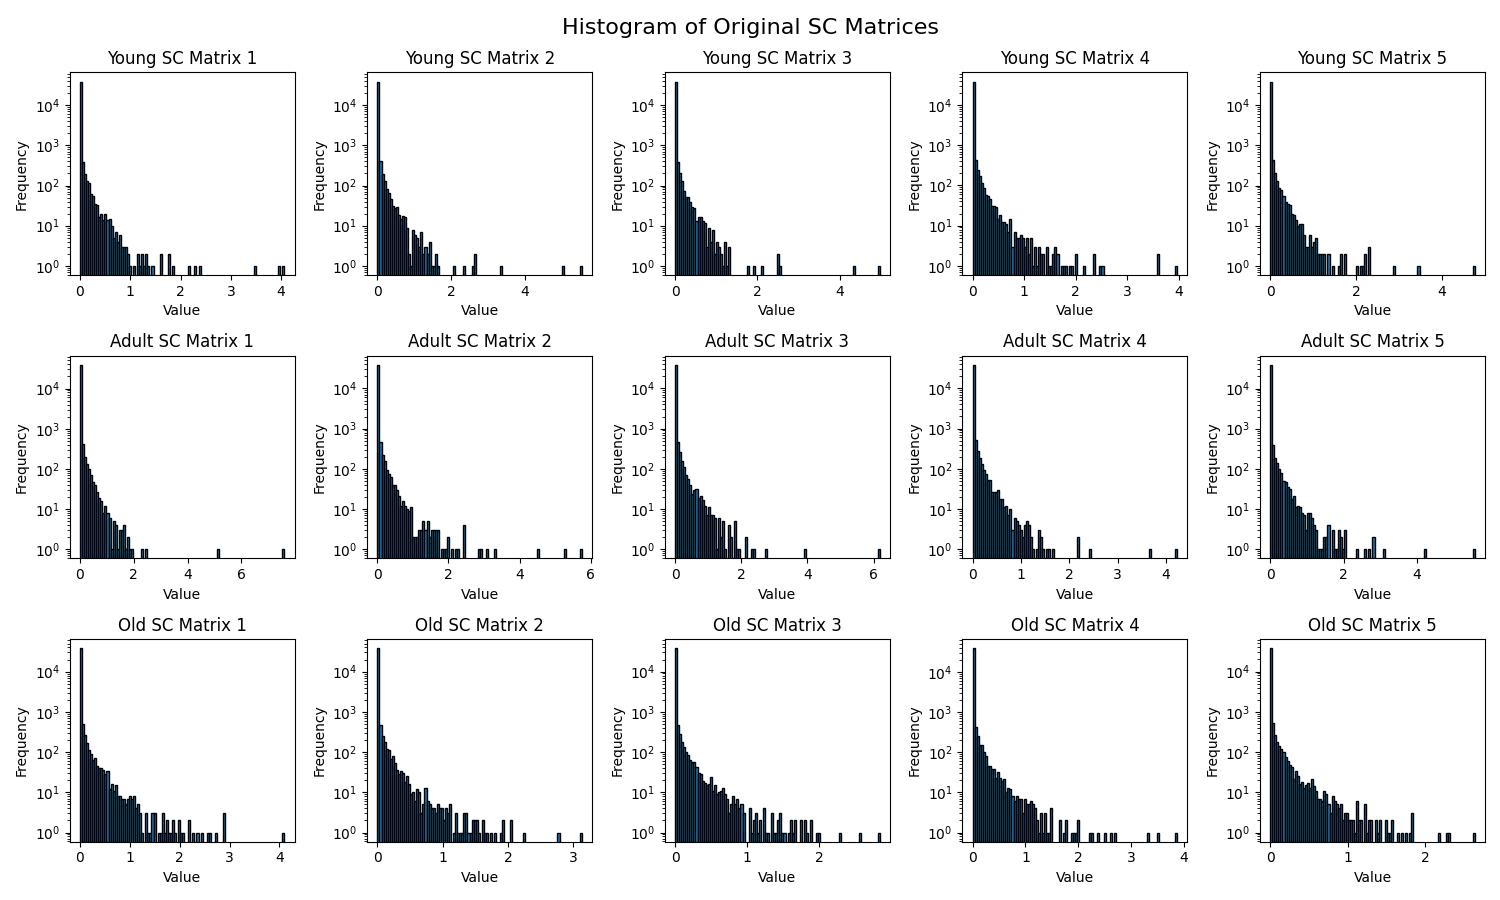
\includegraphics[width=\textwidth]{C:/Users/barbo/Desktop/thesis repo clone/thesis/Thesis Draft/figures/SC_matrices_histogram.png}
        \caption{Histogram of Original SC Matrices}
    \end{subfigure}
    \begin{subfigure}[b]{0.45\textwidth}
        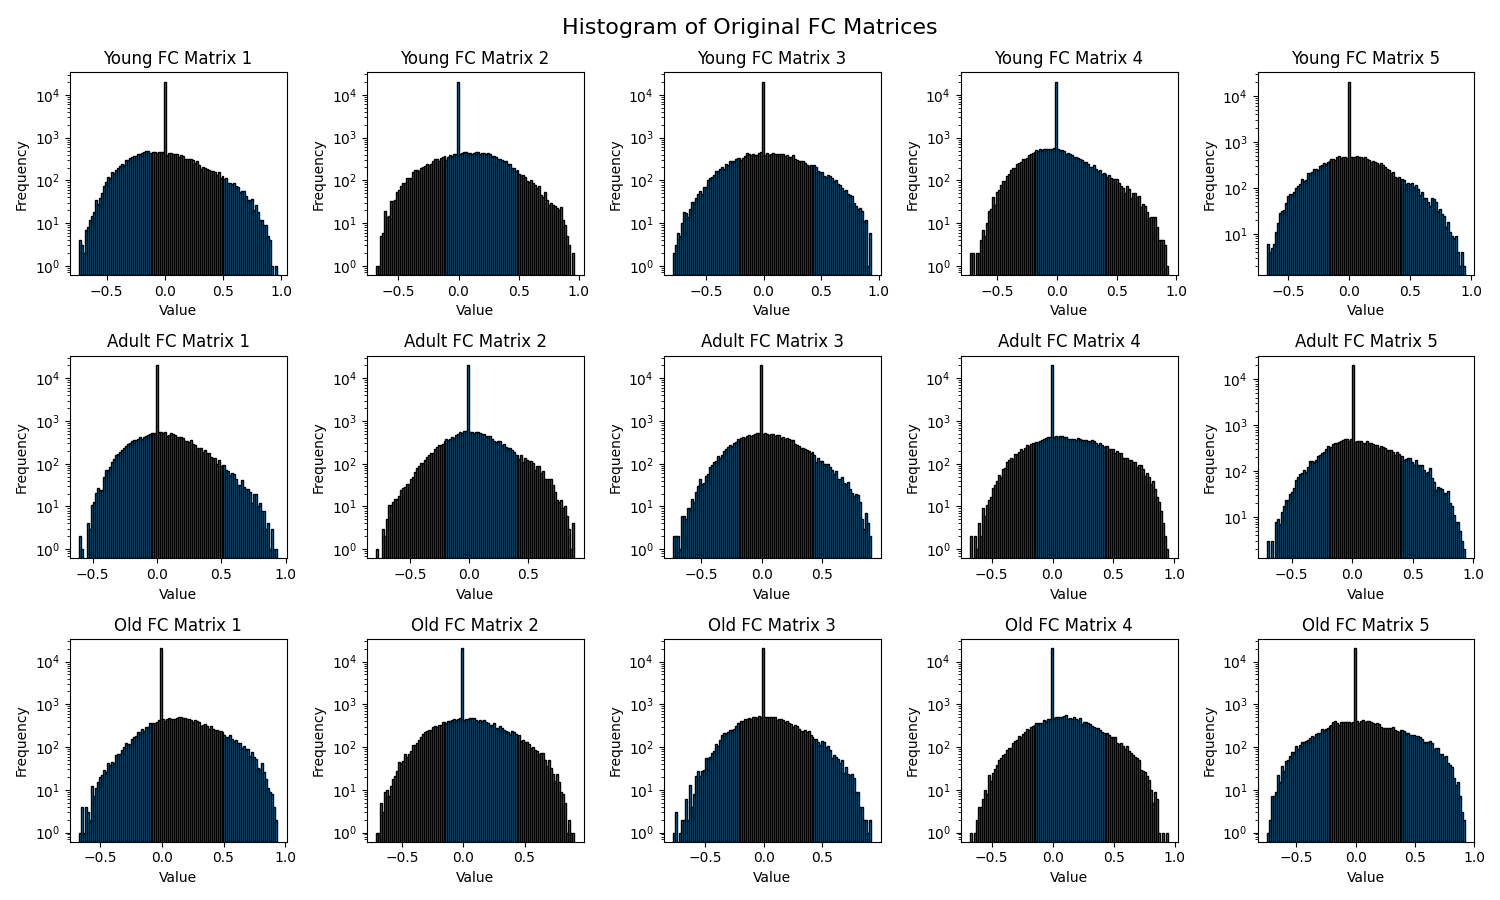
\includegraphics[width=\textwidth]{C:/Users/barbo/Desktop/thesis repo clone/thesis/Thesis Draft/figures/FC_matrices_histogram.png}
        \caption{Histogram of Original FC Matrices}
    \end{subfigure}
    \begin{subfigure}[b]{0.45\textwidth}
        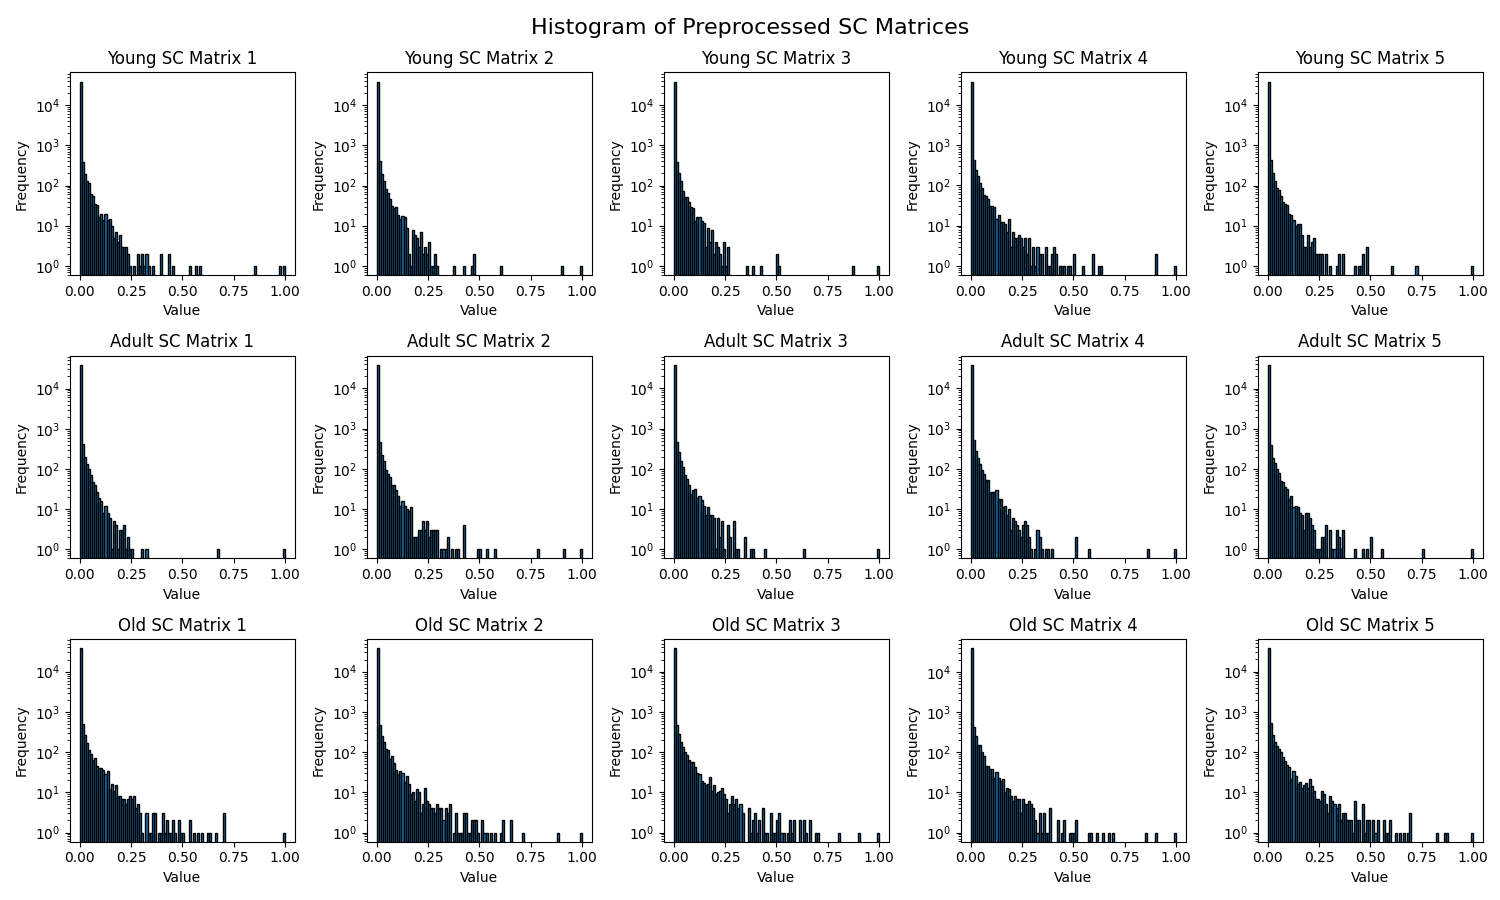
\includegraphics[width=\textwidth]{C:/Users/barbo/Desktop/thesis repo clone/thesis/Thesis Draft/figures/SC_matrices_histogram_preprocessed.png}
        \caption{Histogram of Preprocessed SC Matrices}
    \end{subfigure}
    \begin{subfigure}[b]{0.45\textwidth}
        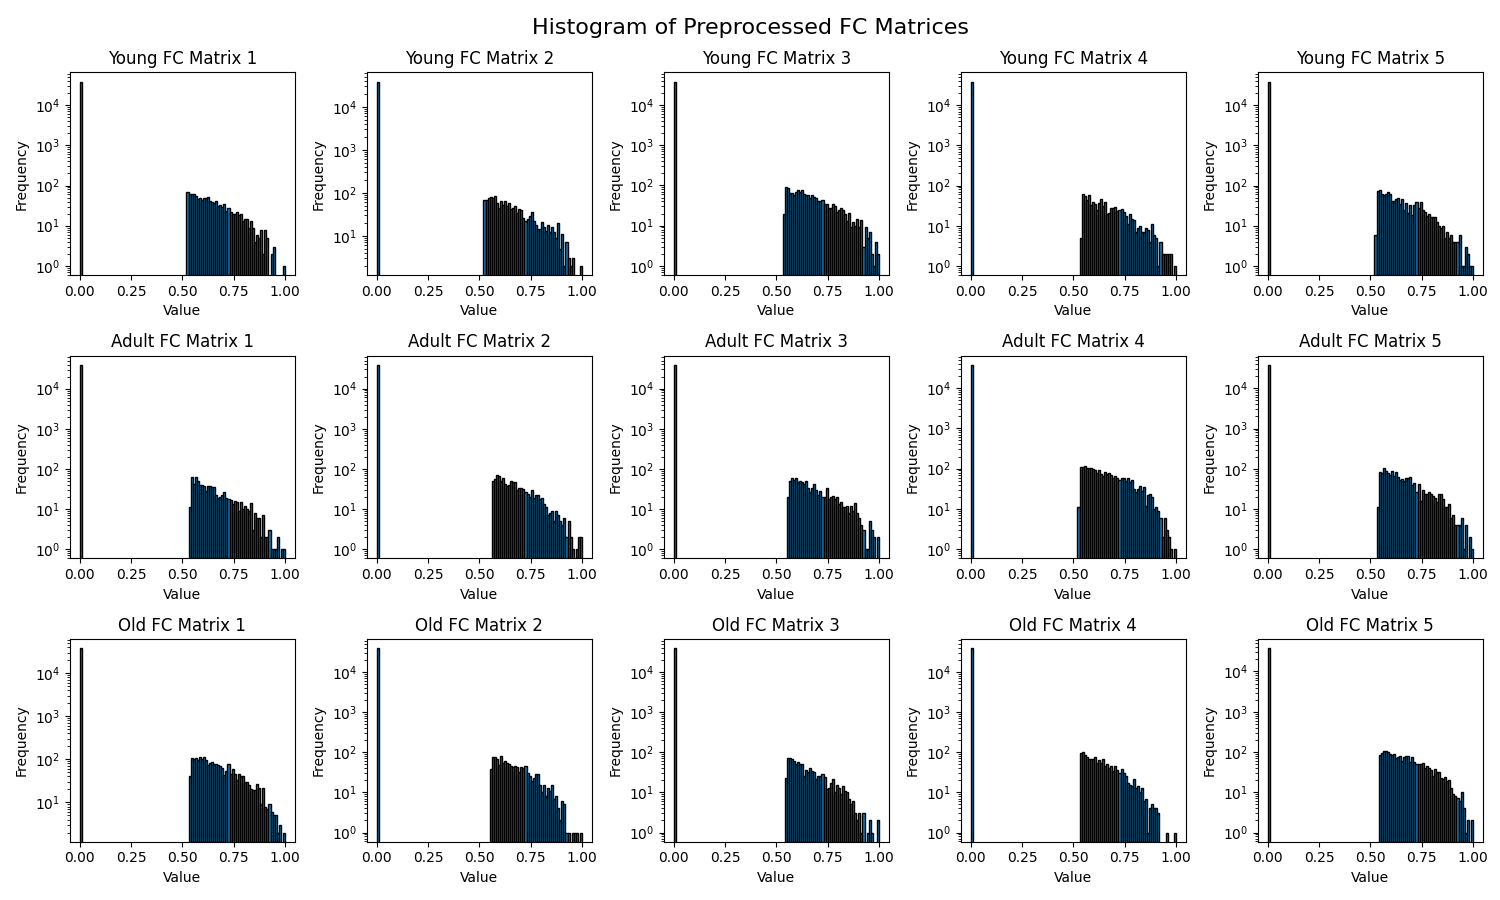
\includegraphics[width=\textwidth]{C:/Users/barbo/Desktop/thesis repo clone/thesis/Thesis Draft/figures/FC_matrices_histogram_preprocessed.png}
        \caption{Histogram of Preprocessed FC Matrices}
    \end{subfigure}
    
    \caption{Various Histograms of SC and FC Matrices}
\end{figure}


\section{Single-Layer Community Detection}
Converted matrices to graphs using \texttt{networkx}. 
Preprocessed graphs by removing self-loops, isolates, and small disconnected components to ensure that Louvain algorithm identifies significant communities.
Applied the Louvain method for community detection on the preprocessed graphs using the \texttt{community} package.
Visualized graphs derived from original and preprocessed SC and FC matrices, as well as graphs prepared for the Louvain algorithm, including those with detected communities. 
Used the spring layout algorithm for graph visualization to position the nodes. Stored the positions to ensure consistent node placement across different figures.

\begin{figure}[h!]
    \centering
    \begin{subfigure}[b]{0.45\textwidth}
        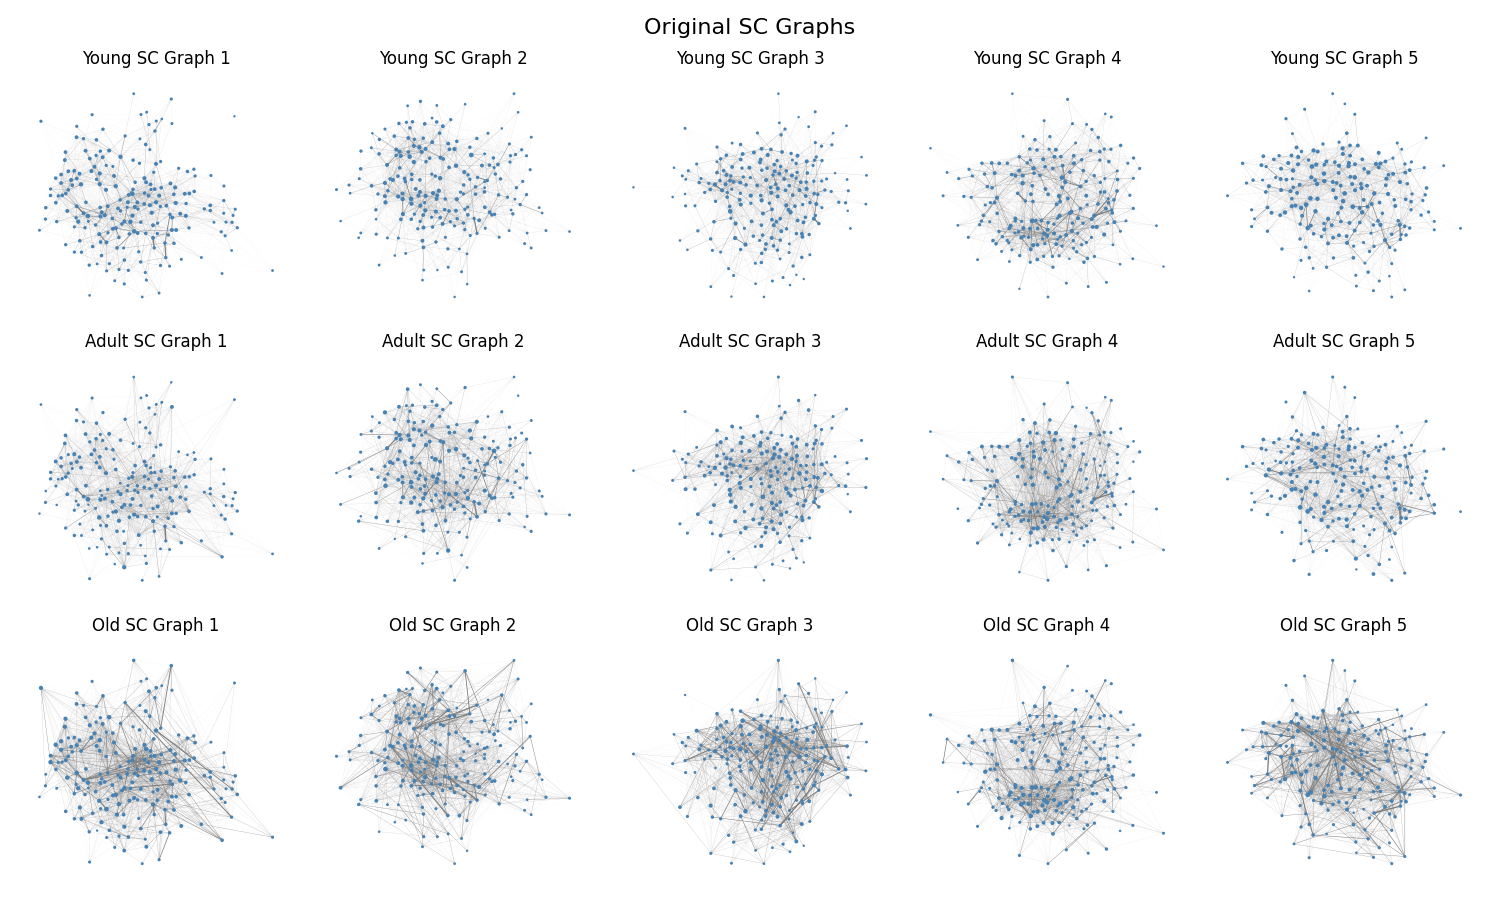
\includegraphics[width=\textwidth]{C:/Users/barbo/Desktop/thesis repo clone/thesis/Thesis Draft/figures/SC_graphs.png}
        \caption{Original SC Graphs}
    \end{subfigure}
    \begin{subfigure}[b]{0.45\textwidth}
        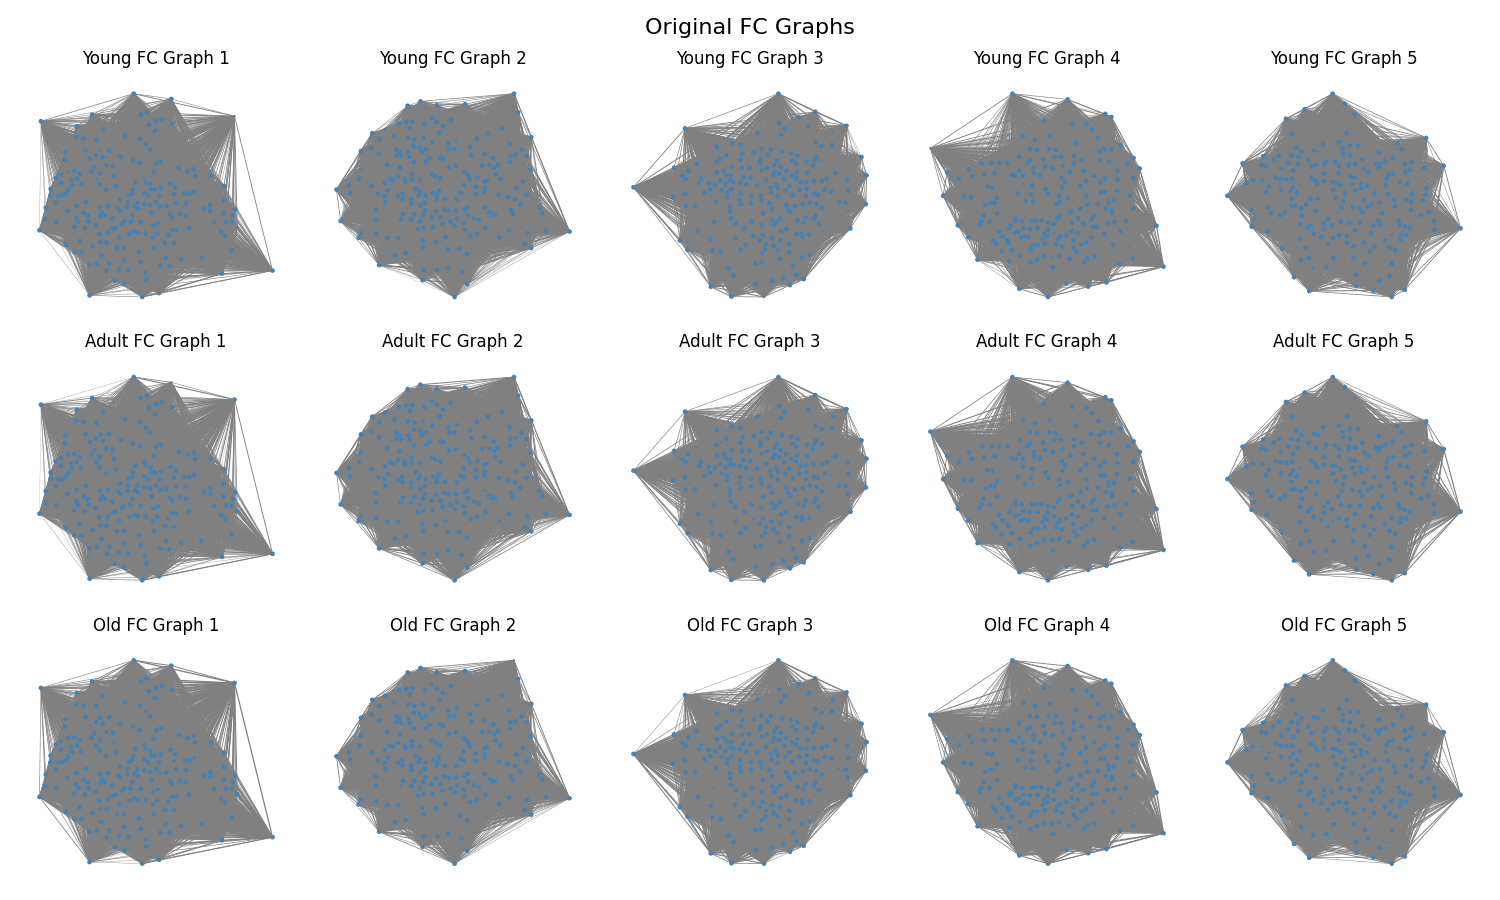
\includegraphics[width=\textwidth]{C:/Users/barbo/Desktop/thesis repo clone/thesis/Thesis Draft/figures/FC_graphs.png}
        \caption{Original FC Graphs}
    \end{subfigure}
    
    \begin{subfigure}[b]{0.45\textwidth}
        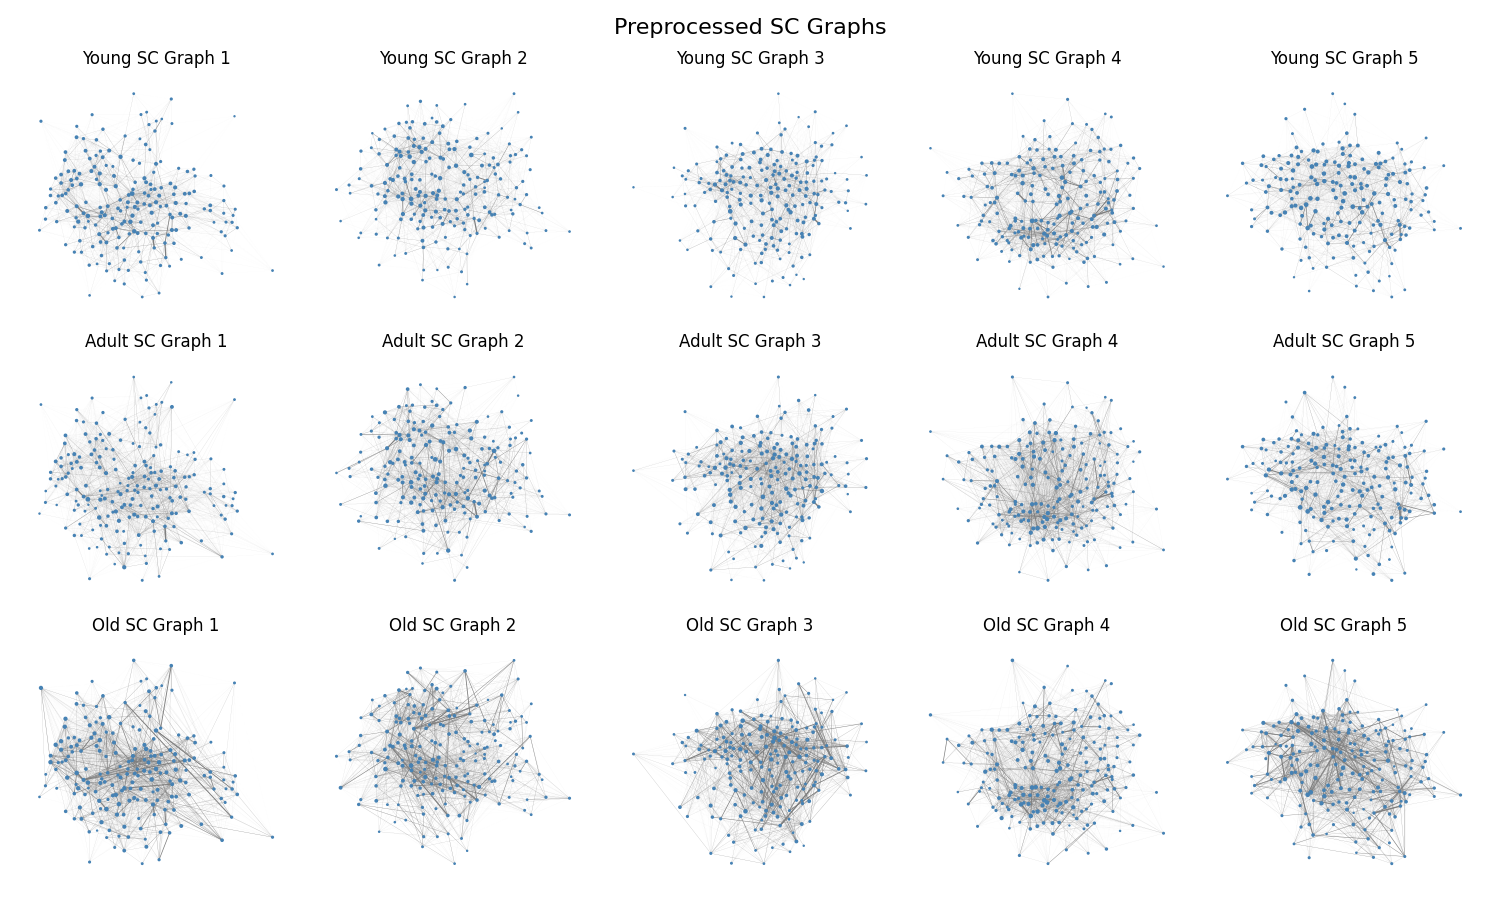
\includegraphics[width=\textwidth]{C:/Users/barbo/Desktop/thesis repo clone/thesis/Thesis Draft/figures/SC_graphs_preprocessed.png}
        \caption{Preprocessed SC Graphs}
    \end{subfigure}
    \begin{subfigure}[b]{0.45\textwidth}
        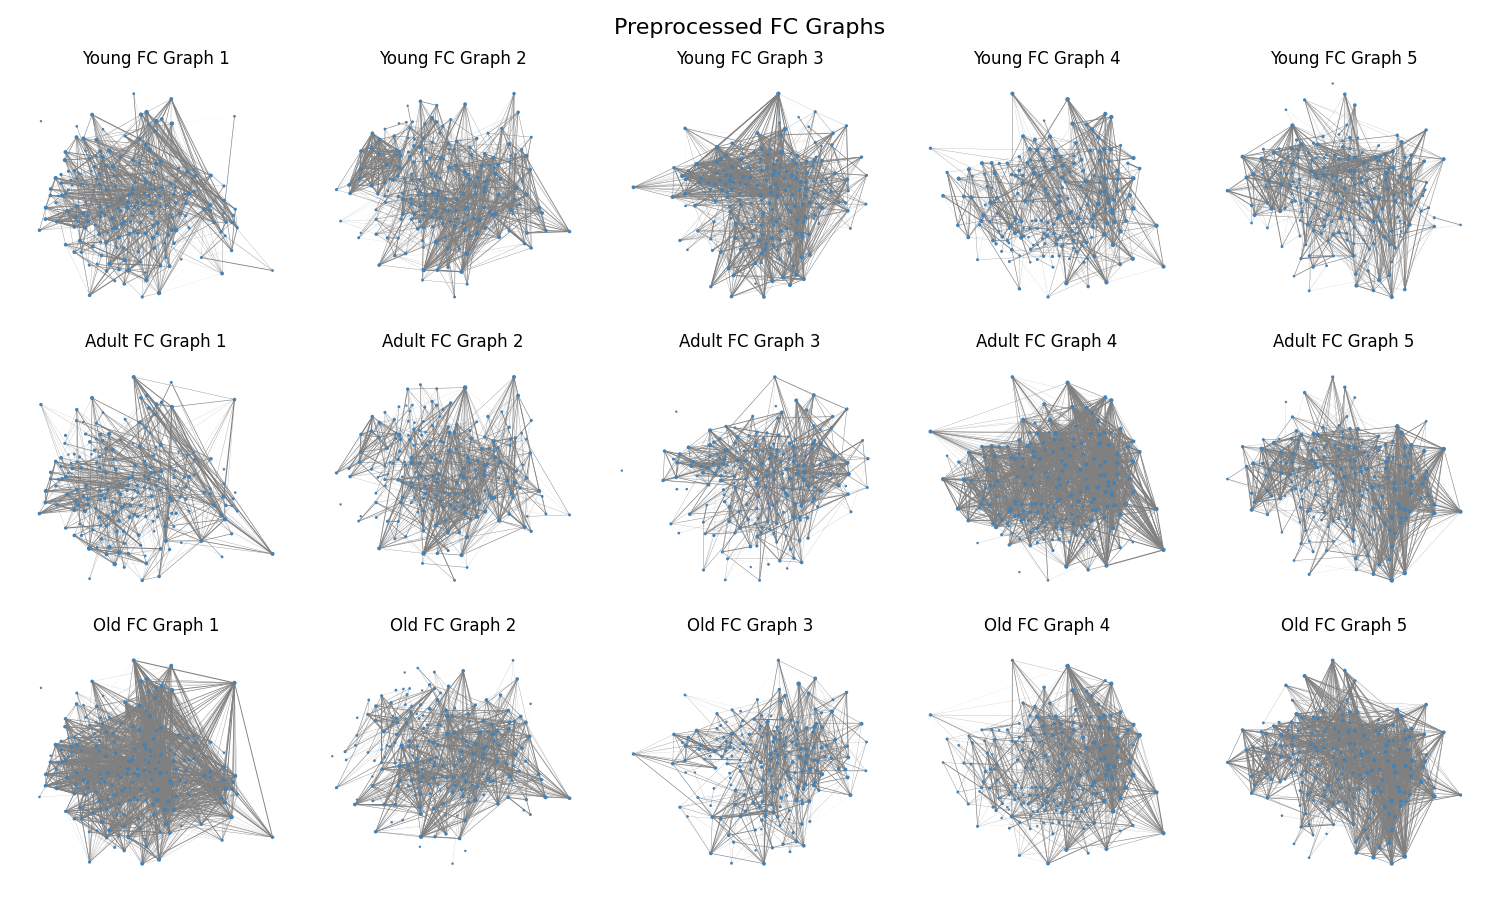
\includegraphics[width=\textwidth]{C:/Users/barbo/Desktop/thesis repo clone/thesis/Thesis Draft/figures/FC_graphs_preprocessed.png}
        \caption{Preprocessed FC Graphs}
    \end{subfigure}
    
    \begin{subfigure}[b]{0.45\textwidth}
        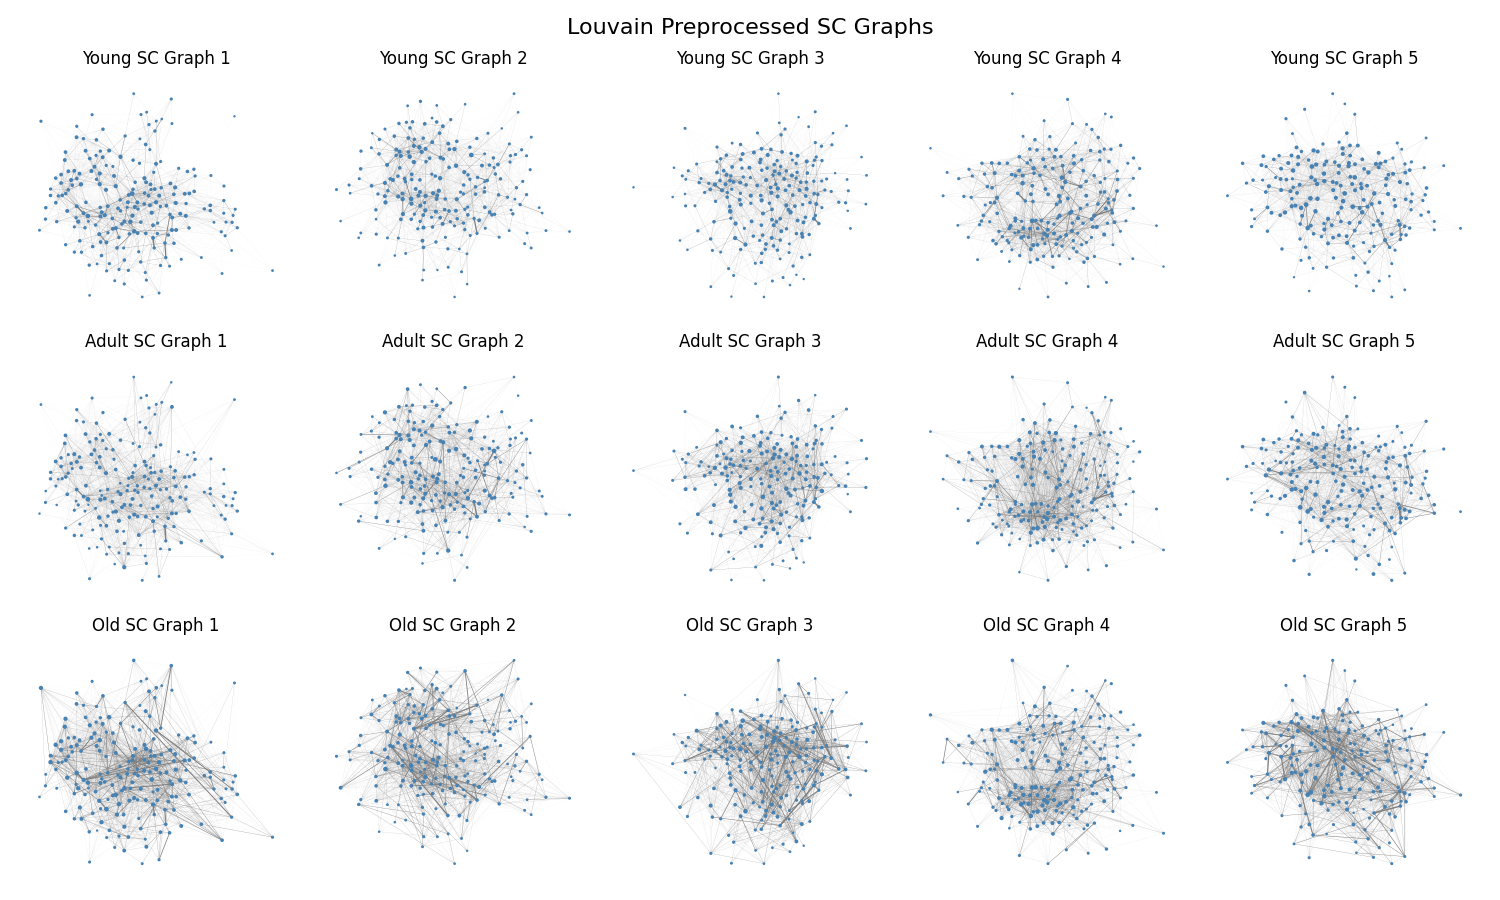
\includegraphics[width=\textwidth]{C:/Users/barbo/Desktop/thesis repo clone/thesis/Thesis Draft/figures/SC_graphs_preprocessed_louvain.png}
        \caption{Louvain Preprocessed SC Graphs}
    \end{subfigure}
    \begin{subfigure}[b]{0.45\textwidth}
        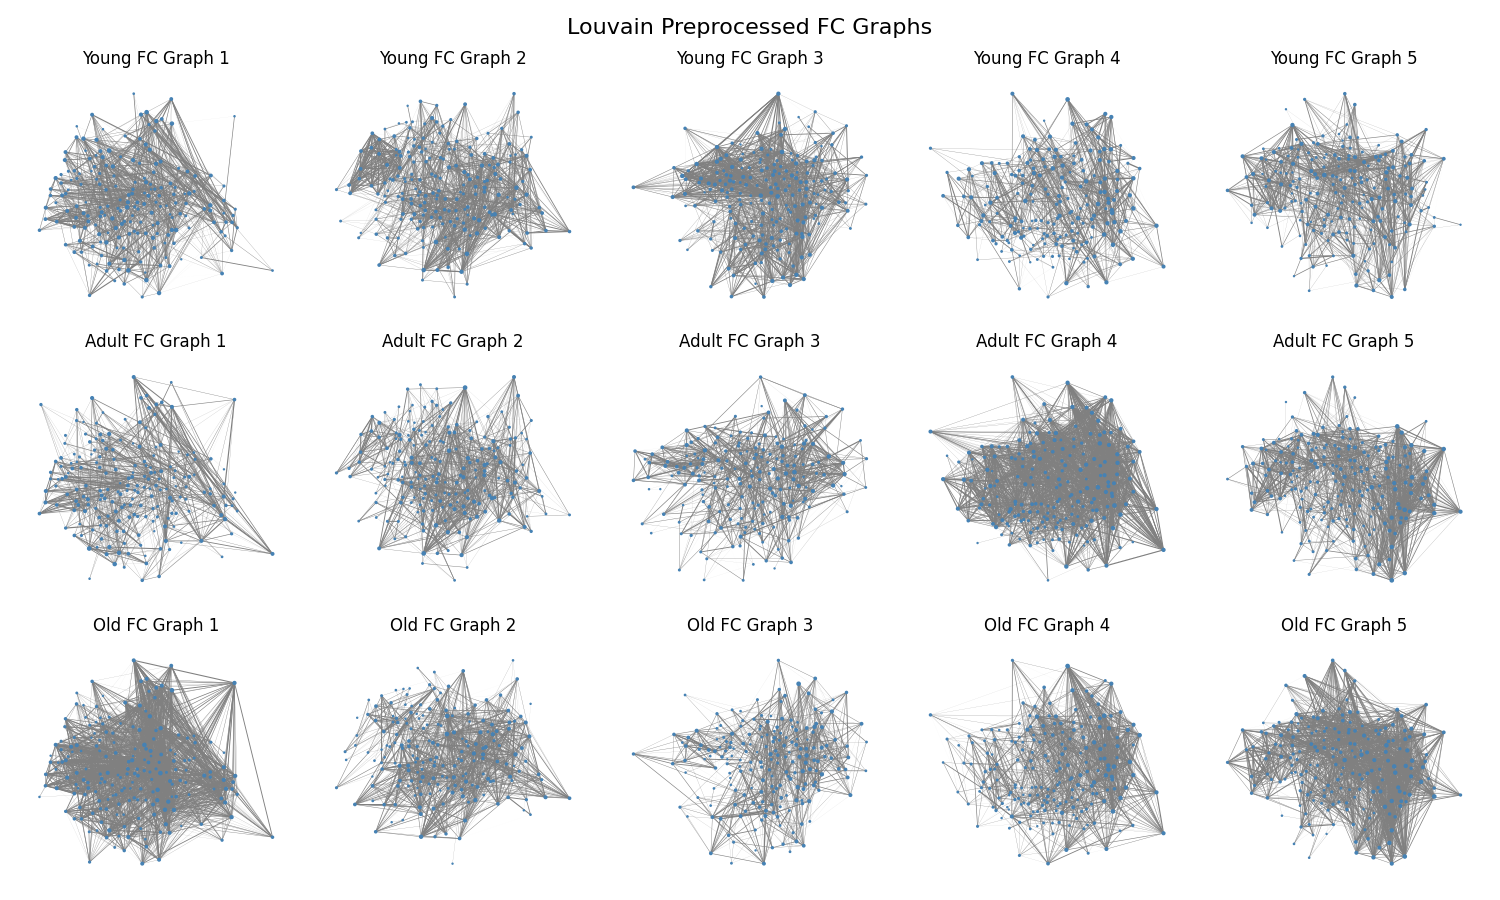
\includegraphics[width=\textwidth]{C:/Users/barbo/Desktop/thesis repo clone/thesis/Thesis Draft/figures/FC_graphs_preprocessed_louvain.png}
        \caption{Louvain Preprocessed FC Graphs}
    \end{subfigure}
    
    \begin{subfigure}[b]{0.45\textwidth}
        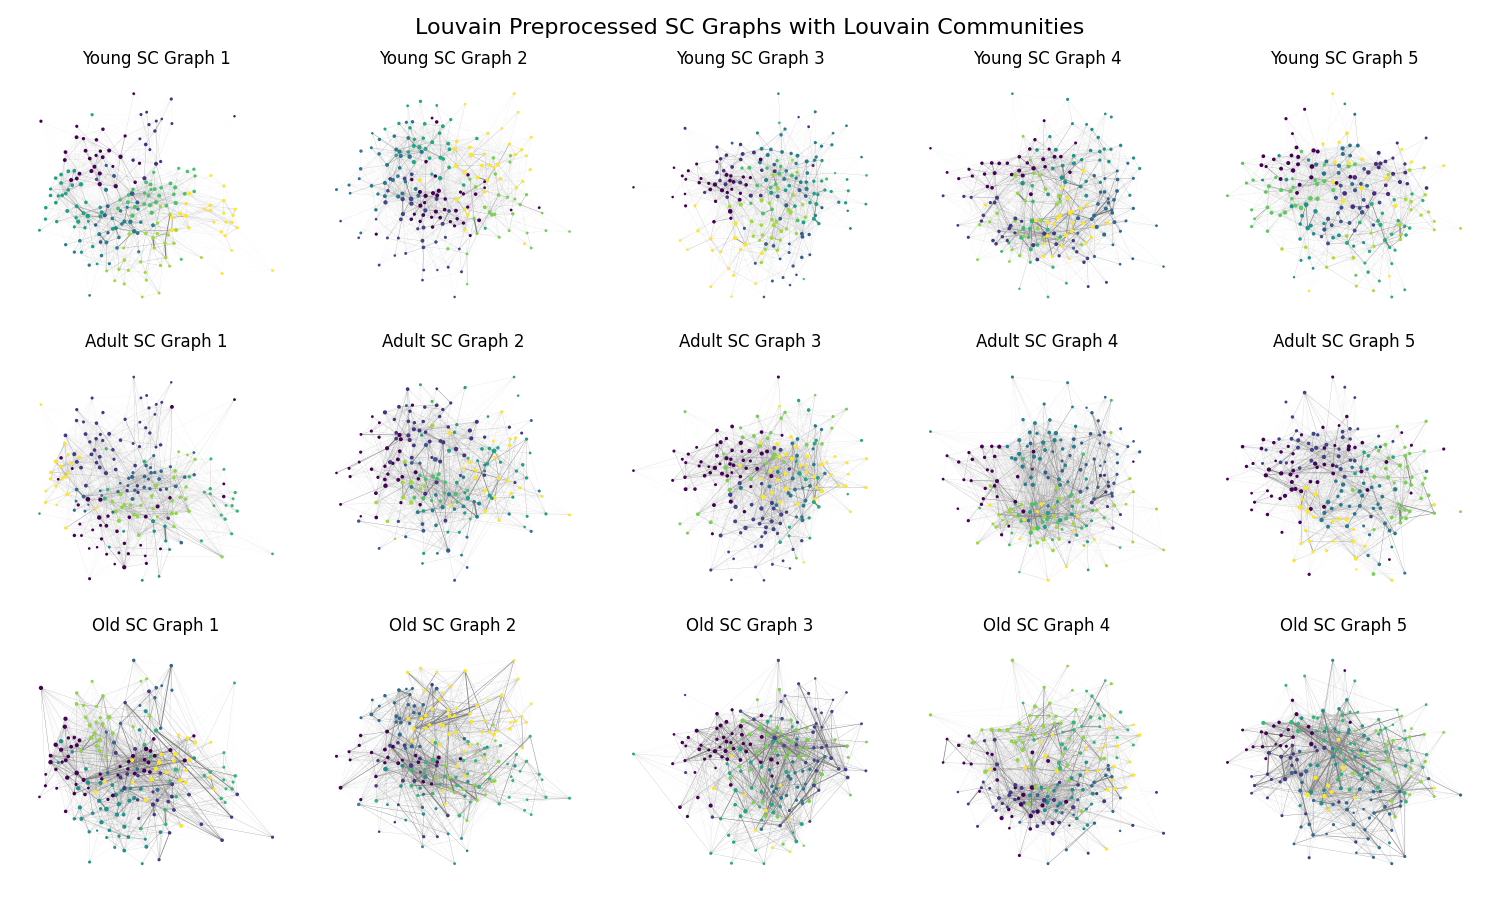
\includegraphics[width=\textwidth]{C:/Users/barbo/Desktop/thesis repo clone/thesis/Thesis Draft/figures/SC_graphs_preprocessed_louvain_communities.png}
        \caption{Louvain Preprocessed SC Graphs with Louvain Communities}
    \end{subfigure}
    \begin{subfigure}[b]{0.45\textwidth}
        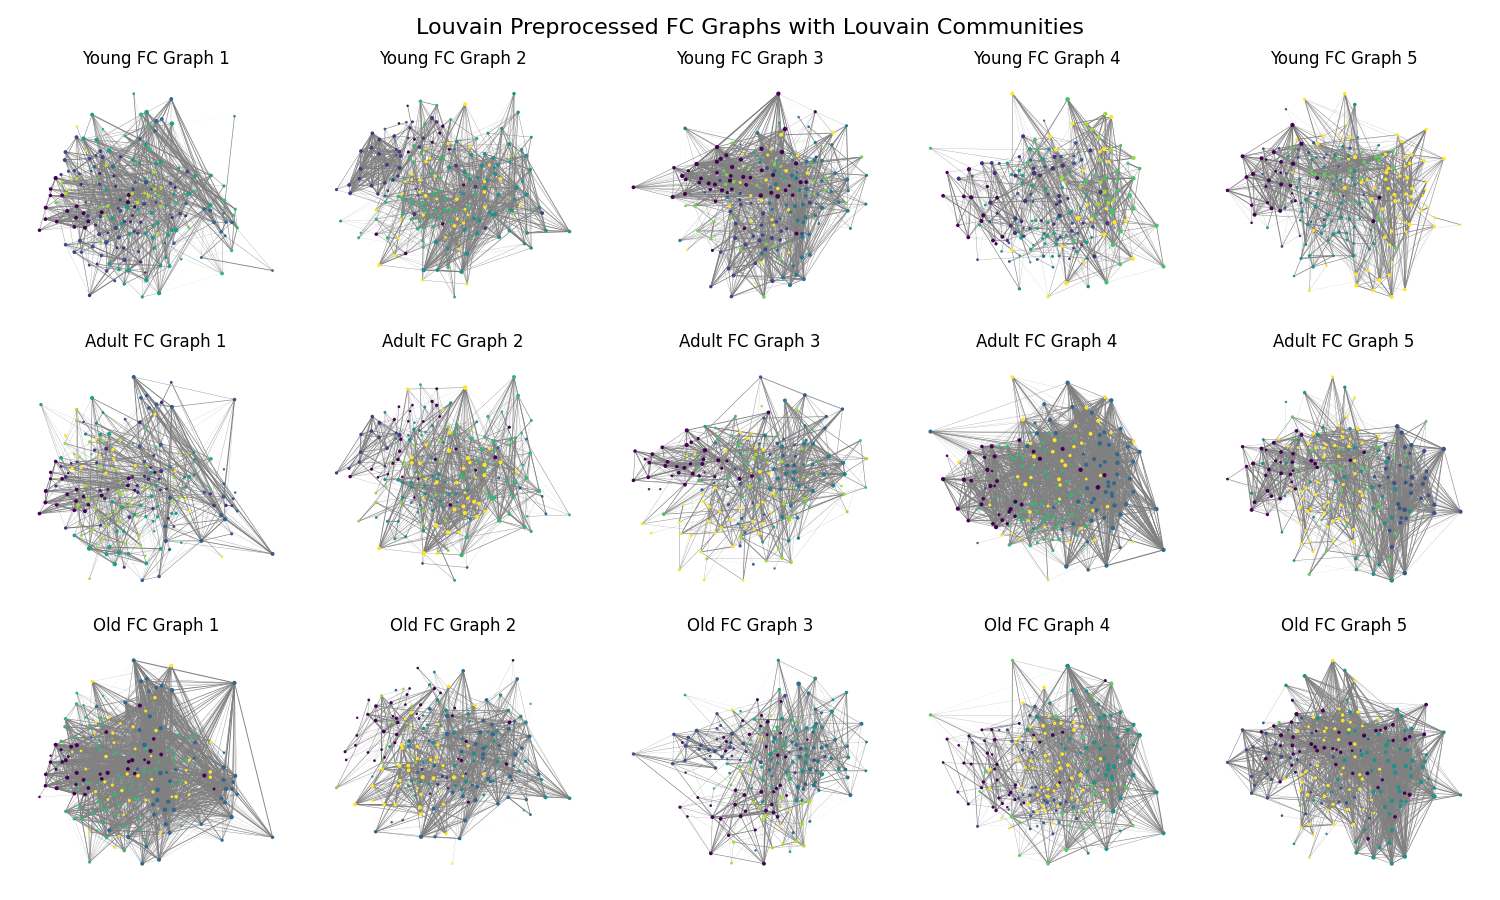
\includegraphics[width=\textwidth]{C:/Users/barbo/Desktop/thesis repo clone/thesis/Thesis Draft/figures/FC_graphs_preprocessed_louvain_communities.png}
        \caption{Louvain Preprocessed FC Graphs with Louvain Communities}
    \end{subfigure}
    
    \caption{Various Graphs of SC and FC Matrices}
\end{figure}






